\documentclass[12pt,a4paper]{extarticle}
\usepackage[left=25mm,right=20mm,top=20mm,bottom=20mm]{geometry}
\usepackage{fontspec}
\IfFontExistsTF{Times New Roman}{\setmainfont{Times New Roman}}{\setmainfont{Liberation Serif}}
\setmonofont{DejaVu Sans Mono}[Scale=0.8]
\usepackage{polyglossia}
\setdefaultlanguage{russian}
\setotherlanguage{english}
\usepackage{amsmath,amssymb,graphicx,booktabs,tabularx,array}
\usepackage{setspace,caption,float,enumitem,titlesec}
\usepackage[unicode,hidelinks]{hyperref}
\hypersetup{pdfauthor={Шешуков Евгений Игоревич},pdflang={ru-RU}}
\setstretch{1.15}
\setlength{\parindent}{1.25cm}
\setlength{\parskip}{3pt}
\setlength{\emergencystretch}{2em}
\setlength{\tabcolsep}{5pt}
\setlength{\intextsep}{8pt}
\renewcommand{\arraystretch}{1.18}
\captionsetup{font=small,labelsep=colon,justification=centering}
\setlist{nosep,topsep=5pt,leftmargin=1.4cm}
\titleformat{\section}{\large\bfseries}{\thesection.}{0.5em}{}
\titleformat{\subsection}{\normalsize\bfseries}{\thesubsection.}{0.5em}{}
\titlespacing*{\section}{0pt}{12pt}{7pt}
\titlespacing*{\subsection}{0pt}{9pt}{4pt}
\setlength{\abovedisplayskip}{7pt}
\setlength{\belowdisplayskip}{7pt}
\widowpenalty=10000
\clubpenalty=10000
\raggedbottom
\newcommand{\code}[1]{\texttt{\small #1}}
\newcommand{\reporttitle}[2]{%
\hypersetup{pdftitle={Лабораторная работа №#1. #2}}
\begin{titlepage}
\begin{center}
{\bfseries БЕЛОРУССКИЙ ГОСУДАРСТВЕННЫЙ УНИВЕРСИТЕТ\par}
\vspace{4mm}
{\bfseries ФАКУЛЬТЕТ ПРИКЛАДНОЙ МАТЕМАТИКИ\par И ИНФОРМАТИКИ\par}
\vspace{4mm}
Кафедра компьютерных технологий и систем
\vspace{34mm}

{\Large\bfseries ОТЧЁТ ПО ЛАБОРАТОРНОЙ\par РАБОТЕ №#1\par}
\vspace{7mm}
{\Large\bfseries «#2»\par}
\vspace{7mm}
Дисциплина: Компьютерная графика\par
\vspace{3mm}
Номер в списке группы: 13
\end{center}
\vspace{24mm}
\hfill\begin{minipage}{0.57\textwidth}
\textbf{Выполнил:}\par
студент 3 курса 2 группы\par
Шешуков Евгений Игоревич\par
\vspace{6mm}
\textbf{Преподаватель:}\par
Каркоцкий Александр Геннадьевич
\end{minipage}
\vfill
\begin{center}Минск, 2026\end{center}
\end{titlepage}
\setcounter{page}{2}}

\begin{document}
\reporttitle{3}{Базовые растровые алгоритмы}

\section{Цель и задание}
Реализовать четыре базовых алгоритма растеризации: пошаговый, ЦДА, Брезенхем для отрезка и Брезенхем для окружности. Приложение должно показывать пиксели на координатной сетке, поддерживать масштабирование и сопровождать построение вычислениями. Дополнительно реализовано сглаживание по двухпиксельной схеме Ву.

\section{Алгоритмы}
\subsection{Пошаговый алгоритм и ЦДА}
Пусть $\Delta x=x_1-x_0$, $\Delta y=y_1-y_0$, $L=\max(|\Delta x|,|\Delta y|)$. В пошаговом методе при $|\Delta x|\ge|\Delta y|$ ведущей является ось $X$:
\begin{equation}
 x_i=x_0+i\operatorname{sign}(\Delta x),\qquad
 y_i=y_0+\frac{\Delta y}{\Delta x}(x_i-x_0),\qquad i=0,\ldots,L.
\end{equation}
Вторая координата округляется до ближайшего целого. Для крутых отрезков оси меняются местами. Совпадающие концы обрабатываются отдельно: результатом становится один пиксель.

В ЦДА обе координаты накапливаются с постоянными приращениями:
\begin{equation}
 x_{i+1}=x_i+\frac{\Delta x}{L},\qquad y_{i+1}=y_i+\frac{\Delta y}{L}.
\end{equation}
Половины округляются вверх. Допуск $10^{-10}$ в функции округления устраняет ошибки накопления вблизи половины для используемого диапазона координат.

\subsection{Брезенхем для отрезка}
Обозначим $a=\max(|\Delta x|,|\Delta y|)$, $b=\min(|\Delta x|,|\Delta y|)$. Начальное решающее значение $d_0=2b-a$. После вывода пикселя выбирается следующий шаг:
\begin{equation}
 d_{i+1}=\begin{cases}
 d_i+2b,&d_i<0\quad\text{(только ведущая ось)},\\
 d_i+2(b-a),&d_i\ge0\quad\text{(обе оси)}.
 \end{cases}
\end{equation}
Направление по каждой оси задаётся знаком её приращения. Поэтому один алгоритм работает во всех восьми октантах. В основном цикле используются целочисленные операции.

\subsection{Брезенхем для окружности}
Вычисляется один октант: $u_0=0$, $v_0=R$, $d_0=3-2R$. Пока $u\le v$, выводятся точки $(\pm u,\pm v)$ и $(\pm v,\pm u)$ со сдвигом на центр $(c_x,c_y)$. Повторы на осях и диагоналях исключаются.
\begin{equation}
 d_{i+1}=\begin{cases}
 d_i+4u_i+6,&d_i<0,\\
 d_i+4(u_i-v_i)+10,&d_i\ge0.
 \end{cases}
\end{equation}
В первом случае меняется только $u\leftarrow u+1$, во втором также $v\leftarrow v-1$. Радиус 0 даёт один пиксель. Квадратные корни и тригонометрия не используются.

\clearpage
\section{Сопроводительные вычисления}
\subsection{Отрезок $(0,0)\to(13,8)$}
Здесь $a=13$, $b=8$, $d_0=3$. При прямом шаге прибавляется 16, при диагональном --- $16-26=-10$. Первые переходы:
\[
 (0,0,3)\to(1,1,-7)\to(2,1,9)\to(3,2,-1).
\]
\begin{table}[H]
\centering\small
\caption{Трассировка отрезка: П --- прямо, Д --- диагональ; $d_i$ до перехода}
\begin{tabular}{rrrrc@{\qquad}rrrrc}\toprule
$i$ & $x_i$ & $y_i$ & $d_i$ & Шаг & $i$ & $x_i$ & $y_i$ & $d_i$ & Шаг\\\midrule
0 & 0 & 0 & 3 & Д & 7 & 7 & 4 & 11 & Д\\
1 & 1 & 1 & -7 & П & 8 & 8 & 5 & 1 & Д\\
2 & 2 & 1 & 9 & Д & 9 & 9 & 6 & -9 & П\\
3 & 3 & 2 & -1 & П & 10 & 10 & 6 & 7 & Д\\
4 & 4 & 2 & 15 & Д & 11 & 11 & 7 & -3 & П\\
5 & 5 & 3 & 5 & Д & 12 & 12 & 7 & 13 & Д\\
6 & 6 & 4 & -5 & П & 13 & 13 & 8 & 3 & ---\\
\bottomrule\end{tabular}

\end{table}
Пошаговый метод и ЦДА дают для этого примера те же 14 пикселей. Например, при $x=4$ точная ордината равна $32/13\approx2.4615$ и округляется до 2. При $x=5$ получаем $40/13\approx3.0769$ и пиксель $(5,3)$. На других отрезках методы могут по-разному разрешать точное попадание между двумя соседними центрами; это не означает ошибку.

\subsection{Окружность с центром $(0,0)$ и радиусом 8}
Начальное значение $d_0=3-16=-13$. В первом переходе прибавляется $4\cdot0+6=6$, поэтому следующее состояние --- $(u,v,d)=(1,8,-7)$.
\begin{table}[H]
\centering\small
\caption{Состояния одного октанта окружности}
\begin{tabular}{rrrrl}\toprule
$i$ & $u_i$ & $v_i$ & $d_i$ & Изменение координат\\\midrule
0 & 0 & 8 & -13 & $u+1$\\
1 & 1 & 8 & -7 & $u+1$\\
2 & 2 & 8 & 3 & $u+1,\;v-1$\\
3 & 3 & 7 & -11 & $u+1$\\
4 & 4 & 7 & 7 & $u+1,\;v-1$\\
5 & 5 & 6 & 5 & $u+1,\;v-1$\\
\bottomrule\end{tabular}

\end{table}
После последней строки $u=6$, $v=5$, условие $u\le v$ перестаёт выполняться. С учётом симметрии получено 44 различных пикселя. Эти значения проверены отдельными тестами и совпадают с таблицей в приложении.

\clearpage
\section{Координатная сетка и интерфейс}
Целочисленная точка $(x,y)$ обозначает \textbf{центр пикселя}. Его область:
\begin{equation}
 \Omega_{xy}=[x-0.5,x+0.5)\times[y-0.5,y+0.5).
\end{equation}
При размере клетки $s$ и экранном начале $(o_x,o_y)$ центр отображается в
\begin{equation}
 X=o_x+sx,\qquad Y=o_y-sy.
\end{equation}
Минус у $y$ переводит направленную вниз экранную ось в математическую ось, направленную вверх. Границы клетки лежат на расстоянии $s/2$ от центра. Оси проходят через центры, линии сетки --- между ними. Пунктирная идеальная фигура использует то же преобразование.

\begin{figure}[H]
\centering
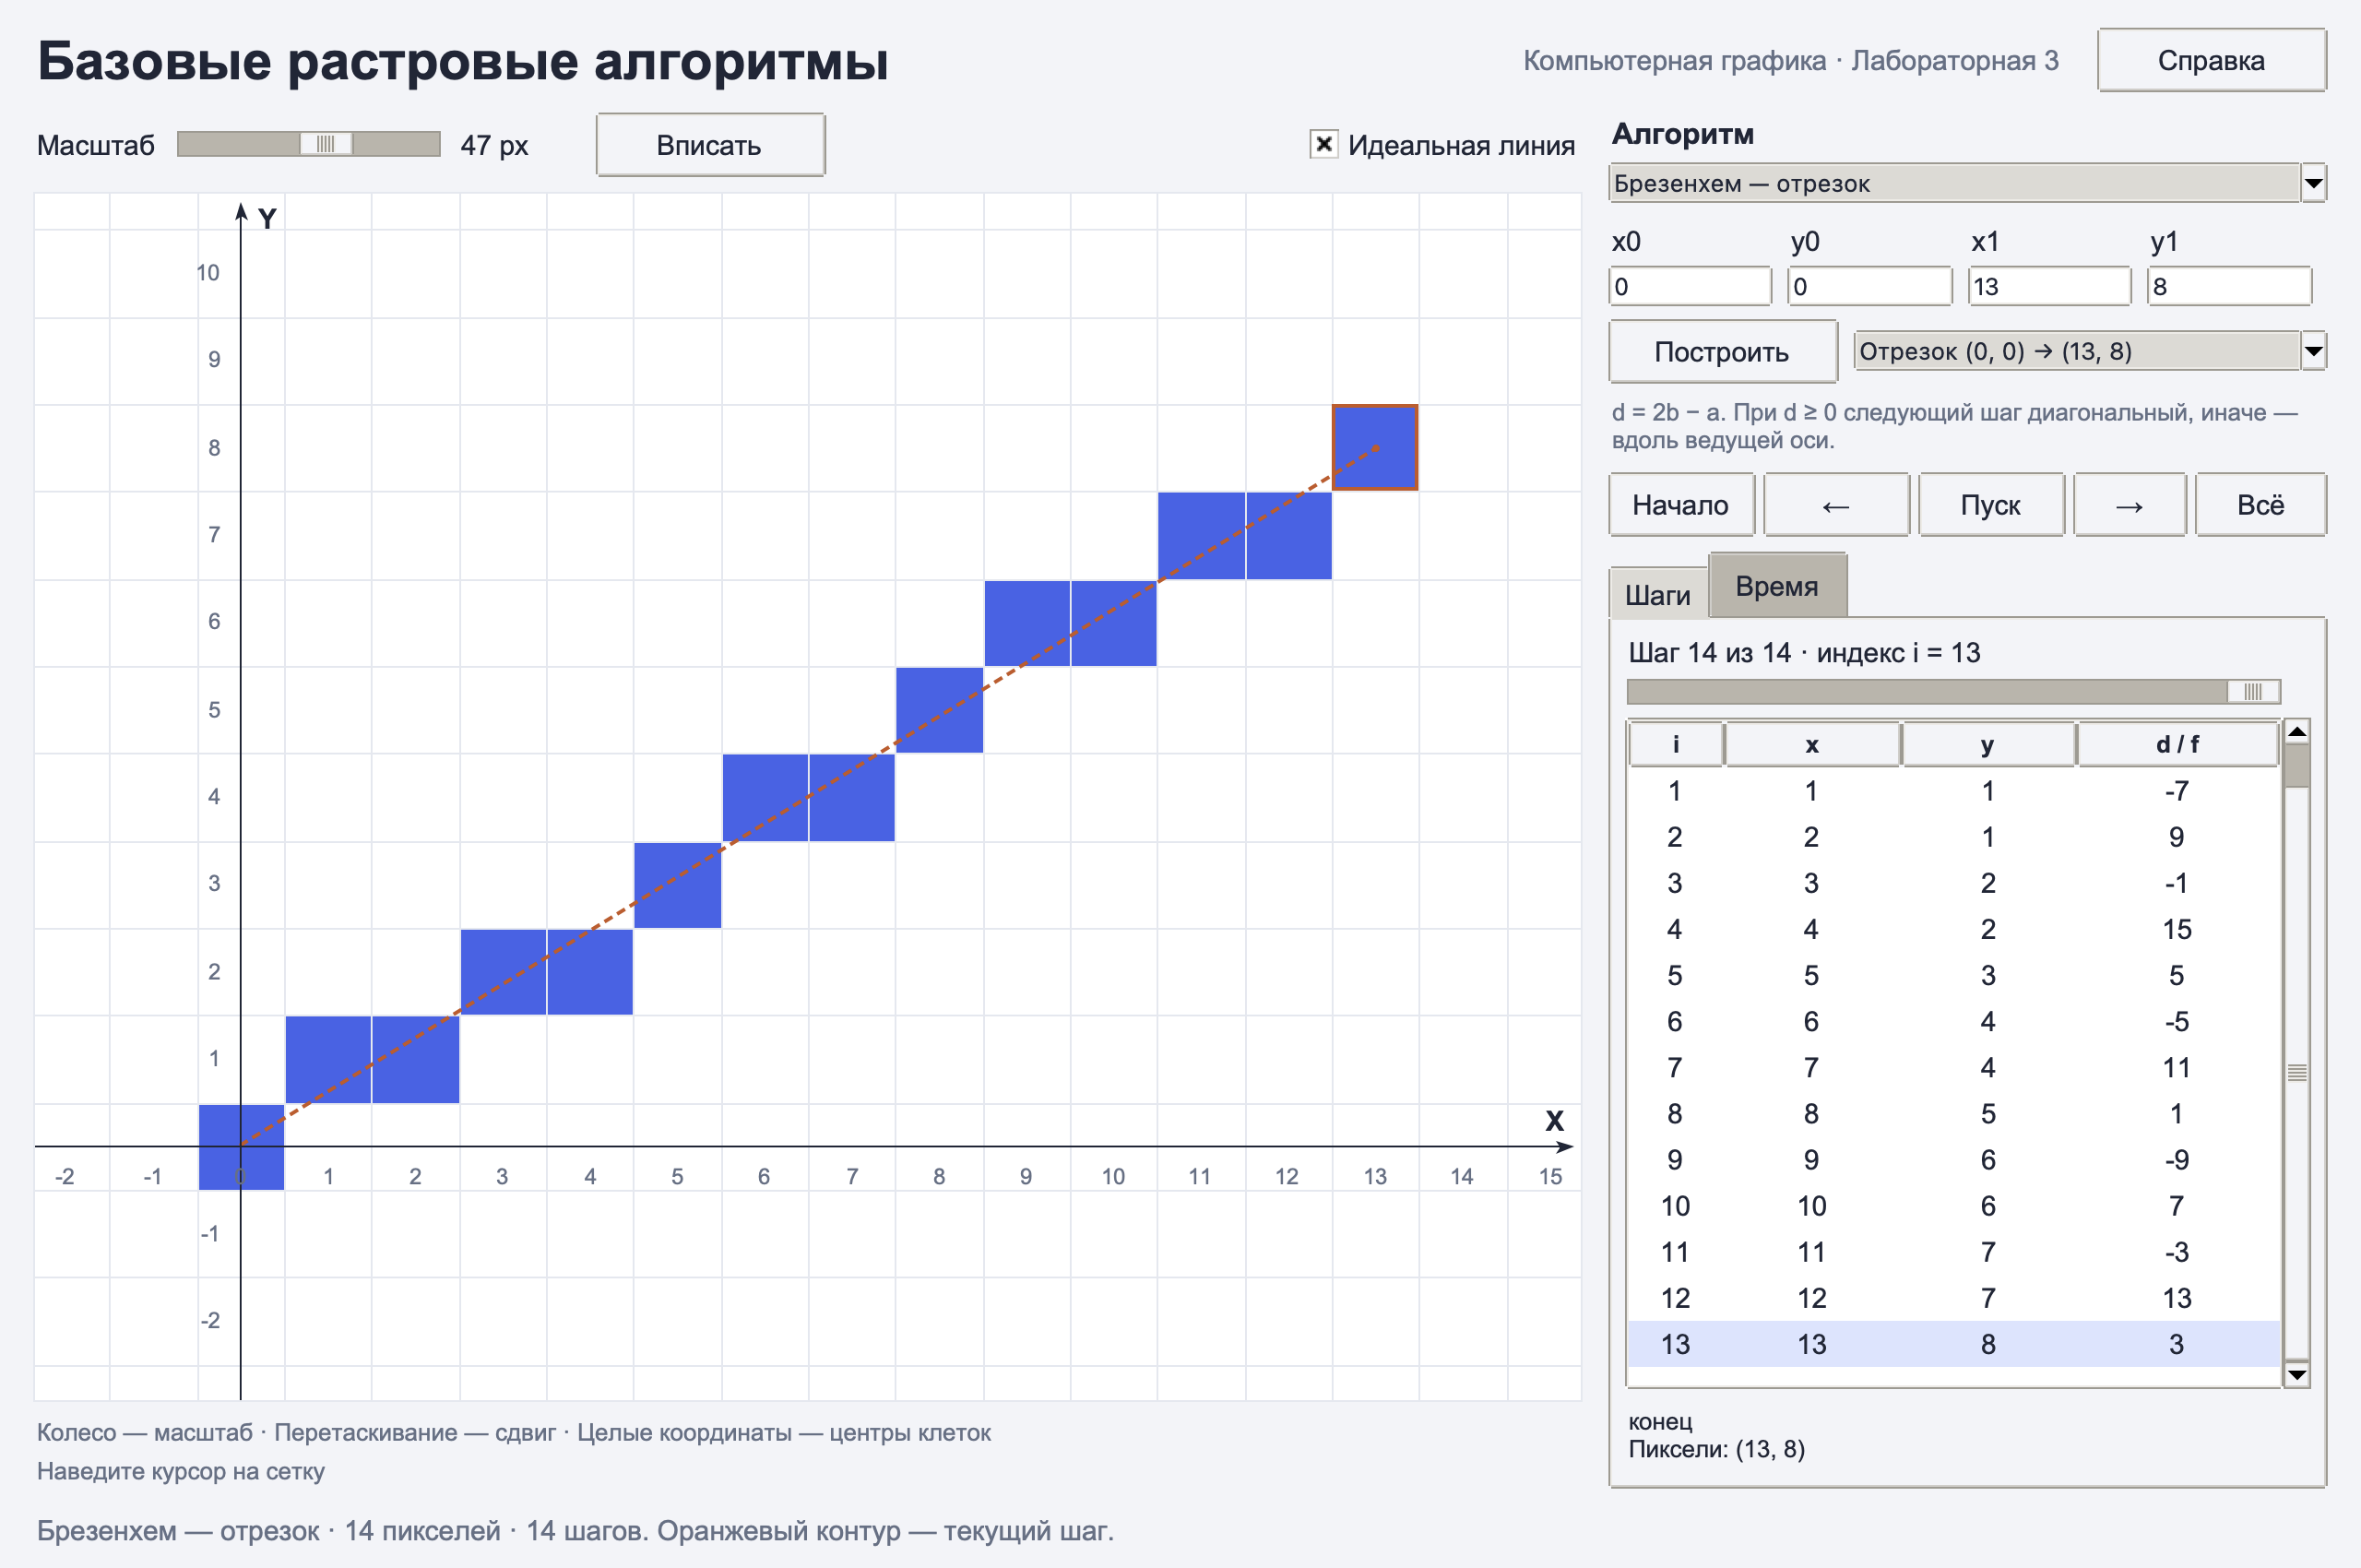
\includegraphics[width=\textwidth]{../docs/line.png}
\caption{Отрезок Брезенхема и таблица его шагов}
\end{figure}
Колесо мыши меняет масштаб около курсора, перетаскивание сдвигает сетку, кнопка «Вписать» показывает фигуру и начало координат. При малом масштабе часть линий сетки и подписей пропускается для читаемости; координаты пикселей при этом не меняются.

Кнопки «Начало», стрелки, «Пуск» и ползунок показывают построение по шагам. Строку можно выбрать в таблице; оранжевые рамки выделяют добавленные на текущем шаге пиксели. Ввод допускает целые координаты от $-1000$ до $1000$ и радиус от 0 до 500. Ошибка ввода сохраняет предыдущий результат и выводит пояснение.

\clearpage
\section{Окружность и сглаженные линии}
\begin{figure}[H]
\centering
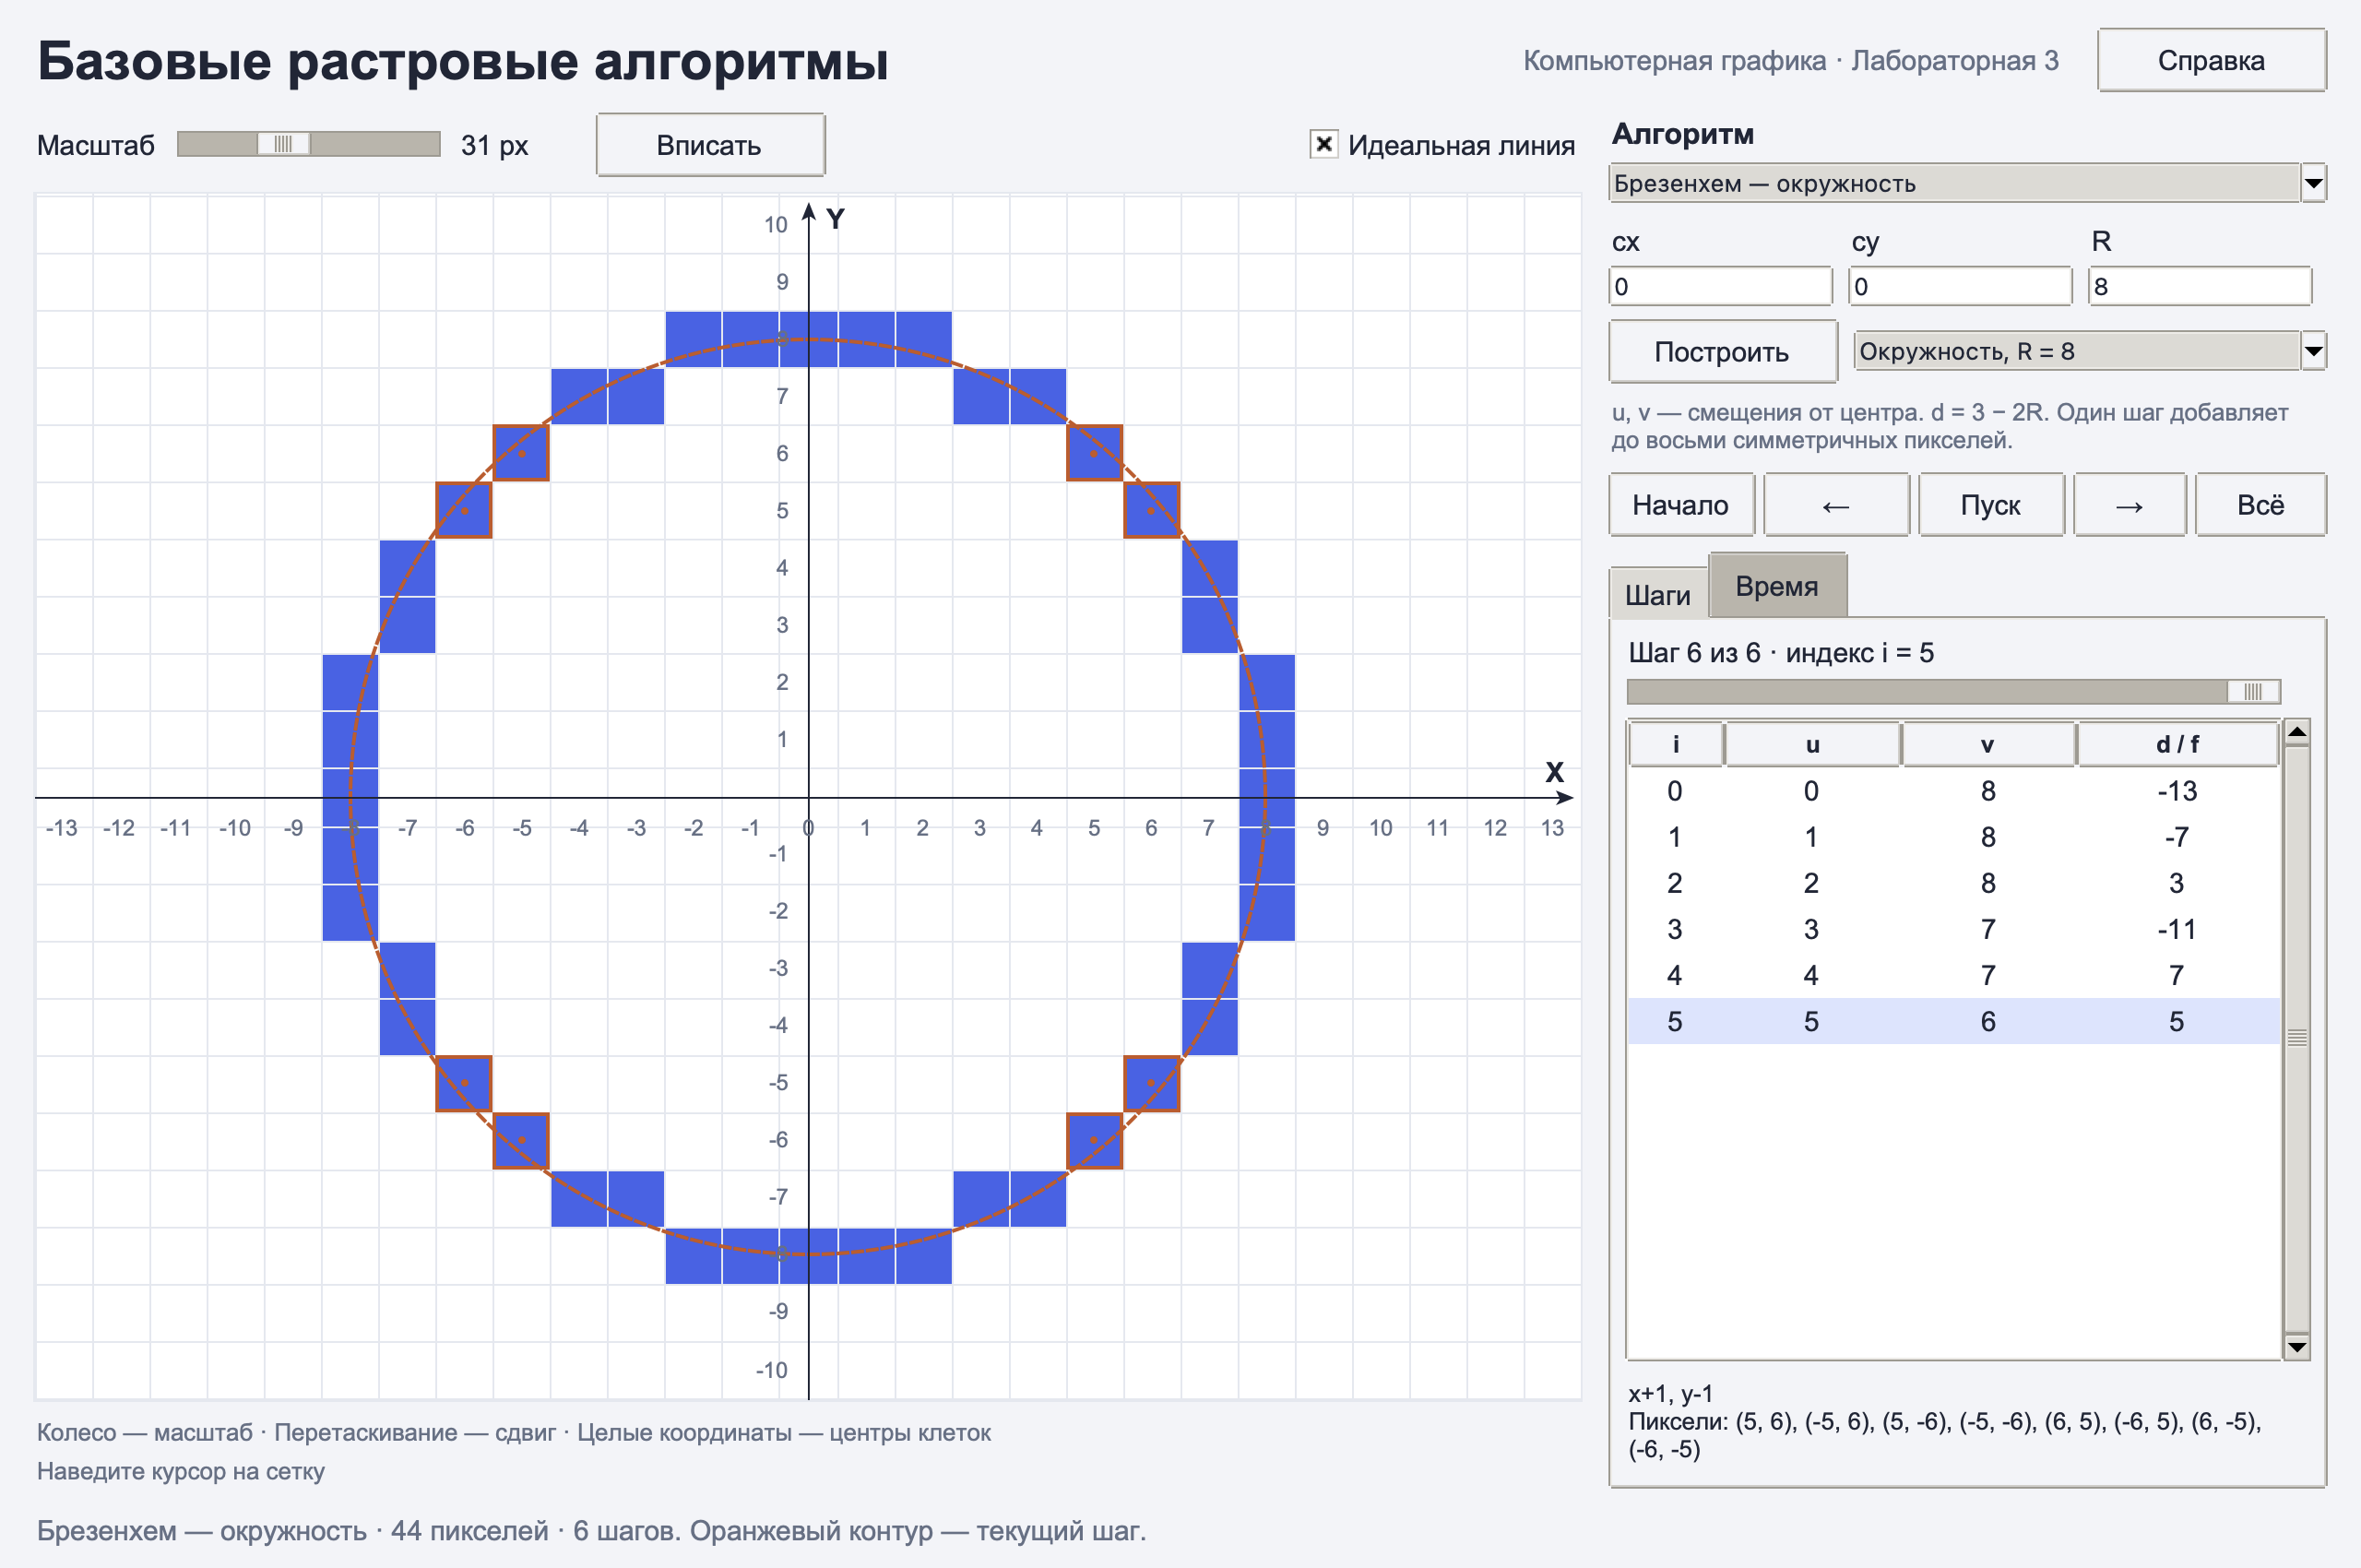
\includegraphics[width=0.72\textwidth]{../docs/circle.png}
\caption{Окружность: один шаг добавляет до восьми симметричных пикселей}
\end{figure}
В дополнительном режиме Ву вместо округления второй координаты $y$ используются два соседних пикселя. Если $j=\lfloor y\rfloor$, $f=y-j$, их веса равны
\begin{equation}
 \alpha(x,j)=1-f,\qquad \alpha(x,j+1)=f.
\end{equation}
Для крутого отрезка оси меняются местами. Сумма весов равна единице, а взвешенная координата совпадает с идеальной линией. Реализован случай целочисленных концов с полностью закрашенными конечными пикселями. Цвет смешивается с белым фоном по весу в экранных RGB-значениях, без гамма-коррекции.
\begin{figure}[H]
\centering
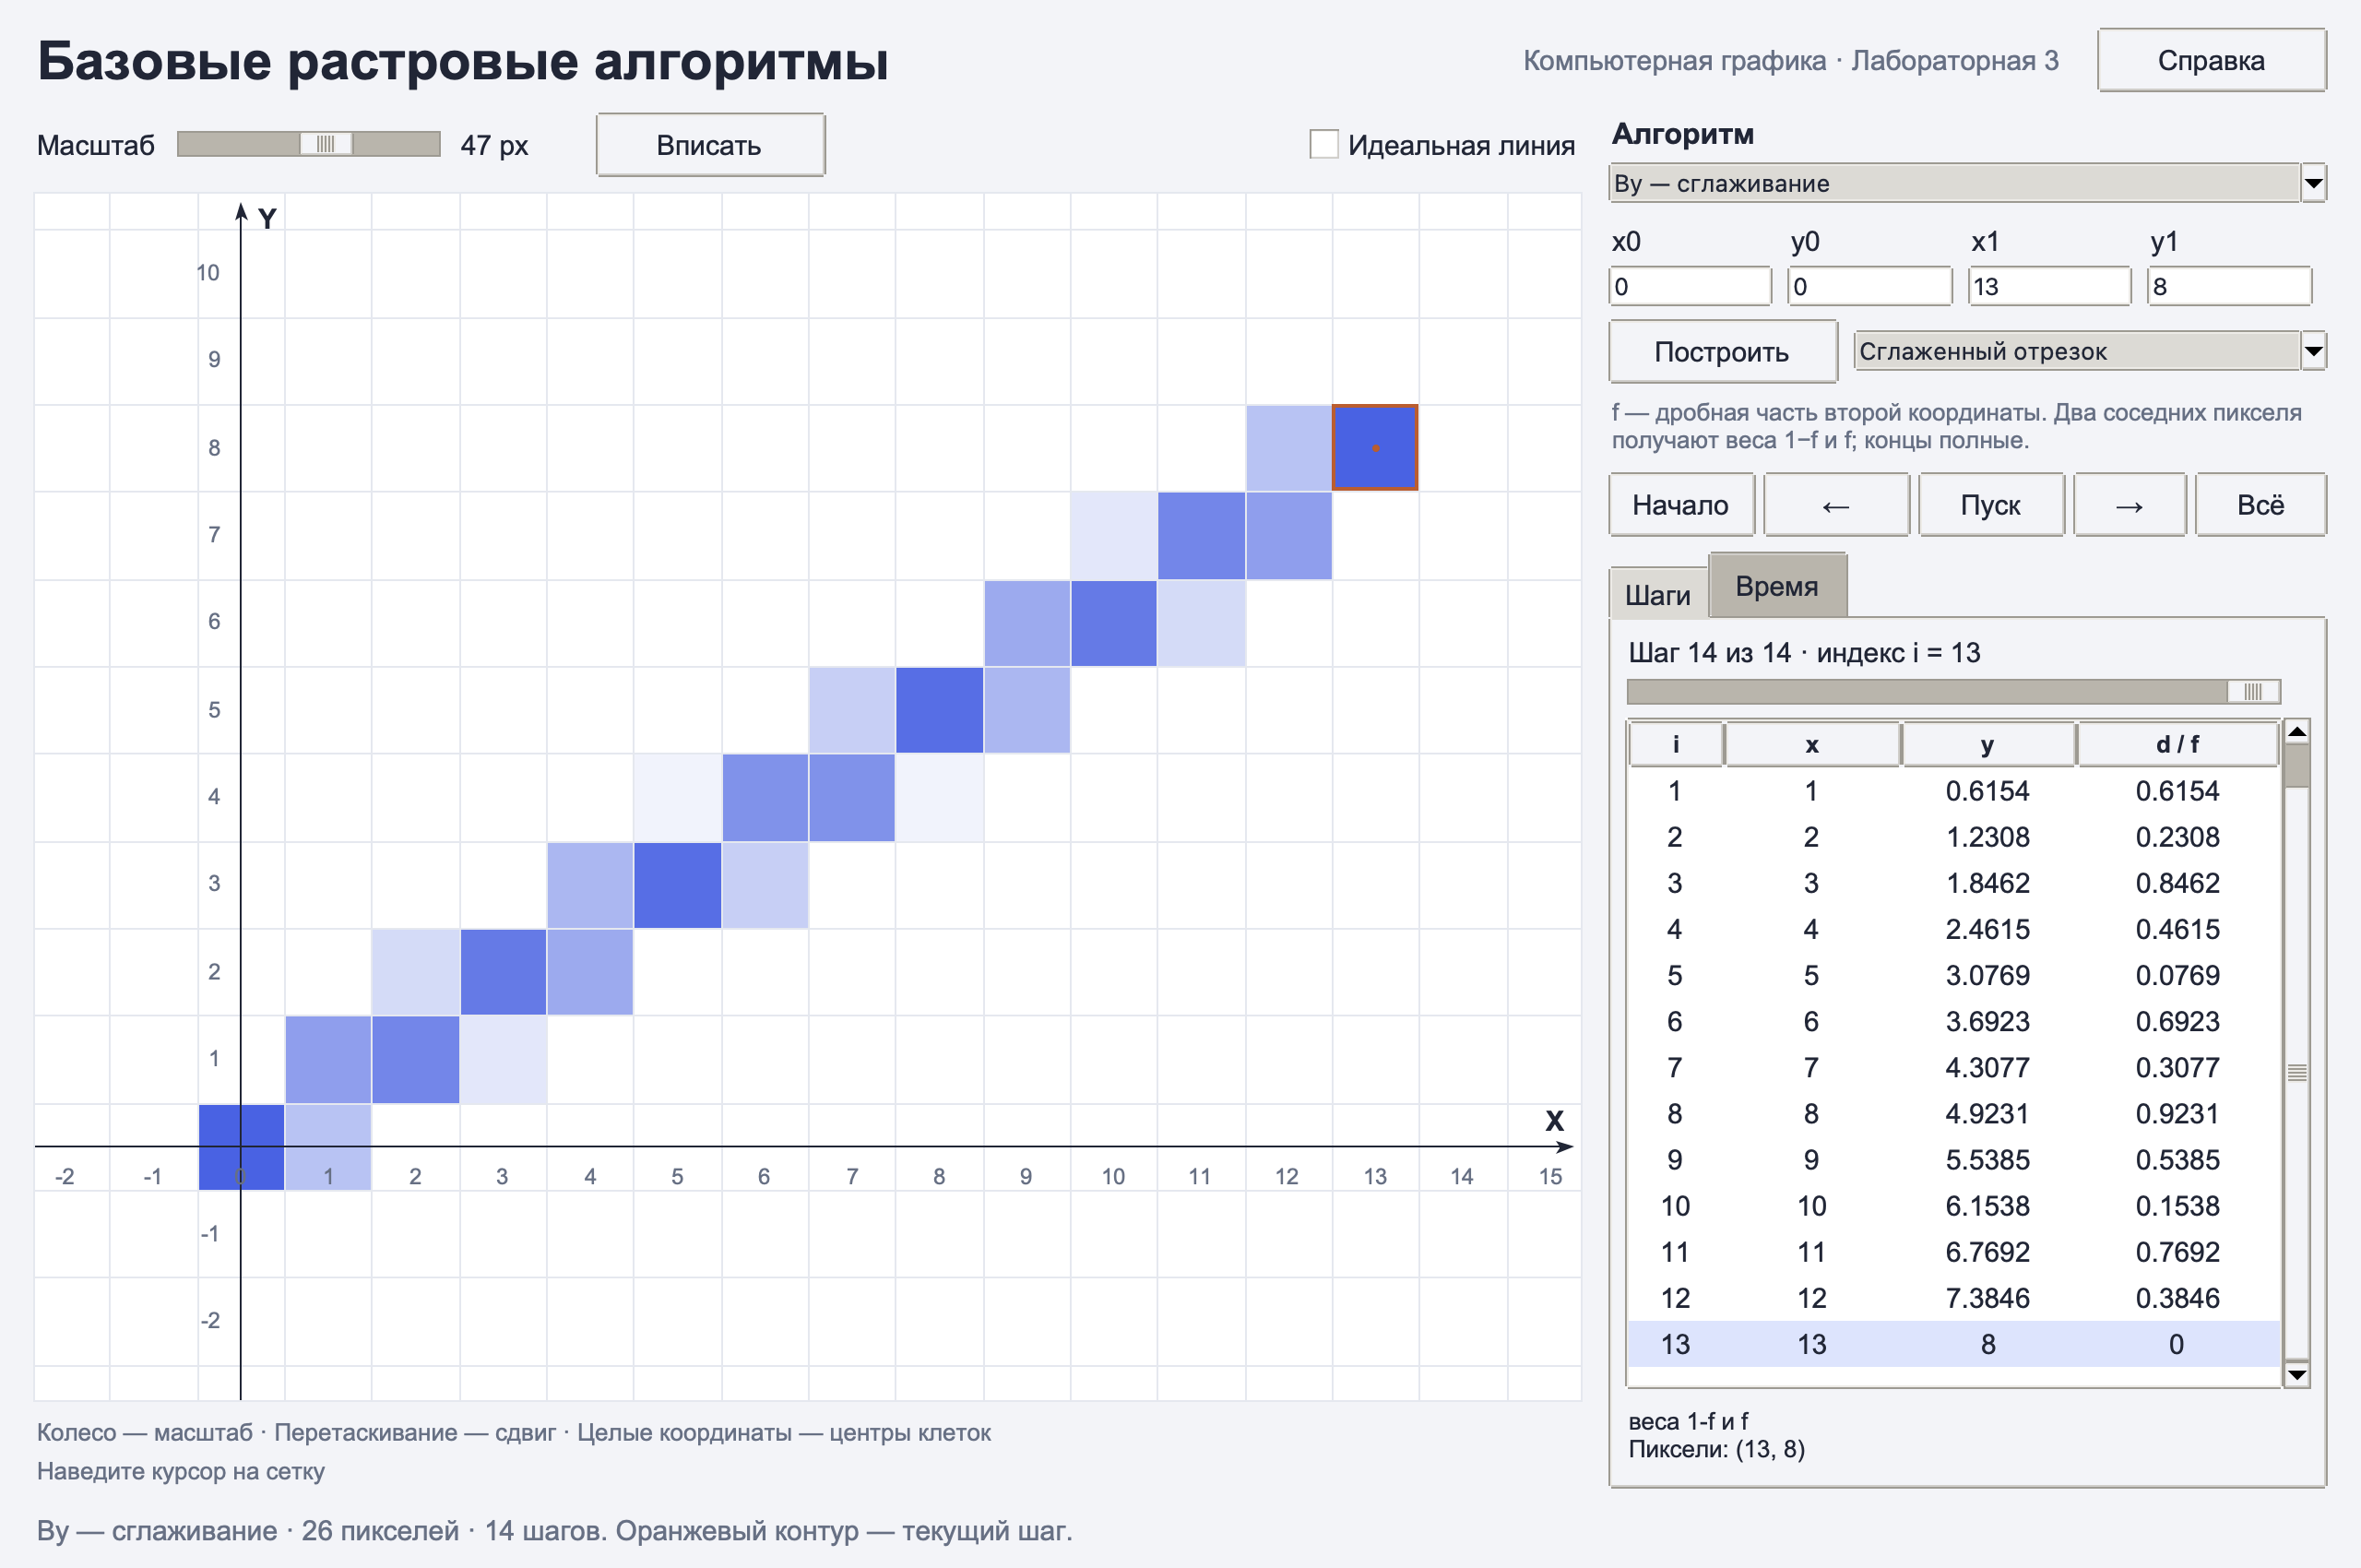
\includegraphics[width=0.72\textwidth]{../docs/wu.png}
\caption{Сглаженный отрезок; пунктир выключен, чтобы видеть веса пикселей}
\end{figure}

\clearpage
\section{Временные характеристики}
Замер выполнен 04.11.2026 в 20:05 (Минск): Apple M3 Pro, Darwin, arm64, Python 3.14.6. Число серий --- 5; повторений набора входов в серии --- 40.


Использован таймер \code{perf\_counter\_ns()}. Измеряется создание полного списка пикселей, включая проверки аргументов и выделение Python-объектов. Отрисовка, сохранение шагов и файловый ввод-вывод исключены. Перед замером выполняется прогрев; сборка циклического мусора отключается на время измеряемого участка.

Для каждой длины отрезка $L\in\{100,500,1000\}$ использованы восемь направлений с отношением меньшего приращения к большему $0.4$. В серии 40 повторений набора, то есть 320 вызовов. Для каждого радиуса окружности выполняются 40 вызовов на серию. В таблицах приведена медиана среднего времени одного вызова по пяти сериям.

\begin{table}[H]
\centering\small
\caption{Время растеризации отрезка, мкс на вызов}
\begin{tabular}{lrrr}\toprule
Алгоритм & $L=100$ & $L=500$ & $L=1000$\\\midrule
Пошаговый & 28.27 & 137.65 & 273.21\\
ЦДА & 23.53 & 119.71 & 235.88\\
Брезенхем — отрезок & 18.87 & 96.28 & 193.06\\
Ву — сглаживание & 51.05 & 249.39 & 501.40\\
\bottomrule\end{tabular}

\end{table}
\begin{table}[H]
\centering\small
\caption{Время растеризации окружности}
\begin{tabular}{rrrr}\toprule
$R$ & Пикселей & Медиана, мкс & Мин.--макс., мкс\\\midrule
40 & 228 & 52.51 & 52.10--54.62\\
200 & 1132 & 261.06 & 255.26--272.45\\
400 & 2264 & 542.92 & 538.94--557.07\\
\bottomrule\end{tabular}

\end{table}
При увеличении длины в 10 раз время приблизительно также увеличивается в 10 раз. Это согласуется с линейной сложностью: $O(L)$ для отрезка и $O(R)$ для окружности. Память под возвращаемый список пикселей тоже линейна.

На измеренных отрезках Брезенхем быстрее пошагового метода и ЦДА. У него нет округления вещественной координаты на каждом шаге. Ву выполняет расчёт весов и создаёт больше пикселей: например, при $L=1000$ получается 1801 пиксель вместо 1001. Поэтому больший расход времени здесь связан в том числе с другим объёмом результата.

Окружность сравнивается отдельно: за итерацию она добавляет до восьми симметричных точек и исключает дубликаты через множество. Абсолютные значения относятся к данной реализации Python и указанным входам. Они могут измениться на другом компьютере или при иной нагрузке. Исходные замеры, минимум, максимум и время на пиксель сохранены в \code{benchmark\_results.json}.

\clearpage
\section{Реализация, проверка и запуск}
Приложение написано на Python с Tkinter; сторонние пакеты не требуются. Файл \code{raster.py} содержит алгоритмы, \code{app.py} --- интерфейс, \code{benchmark.py} --- измерения времени. Растровая фигура рисуется отдельными прямоугольниками найденных пикселей; встроенные линии и окружности Canvas используются только для сетки, осей и идеального контура.

Пройдено 20 тестов: 11 для вычислений и 9 для интерфейса. Проверены все октанты, 100 случайных отрезков с координатами до $1000$ по модулю, концы отрезков, длина списков, связность, вырожденные случаи и расстояние пикселей до идеальной линии. Для радиусов от 1 до 80 проверены симметрия, связность и ошибка окружности. Отдельно проверены ручные трассировки и сумма весов Ву.

Проверки интерфейса выполнялись в настоящем окне Tkinter. Они охватывают выбор шага, переключение режимов, обработку неверного ввода, масштабирование около курсора, сдвиг, вписывание большой фигуры, анимацию, фоновый замер и сохранение результата. Элементы управления проверены при минимальном размере окна $1120\times780$.

Для запуска нужно открыть папку \code{labs/lab03} и дважды щёлкнуть по файлу запуска: \code{run.command} на macOS или \code{run.bat} на Windows. Ручной запуск: \code{python3 app.py} (Windows: \code{py app.py}). Требуется Python 3.10 или новее с Tkinter.

Замеры повторяются командой \code{python3 benchmark.py}. Таблицы отчёта обновляет скрипт \code{report/make\_tables.py}. Для сборки PDF из папки \code{report} выполняется \code{tectonic report.tex}.

\section{Выводы}
Реализованы четыре обязательных алгоритма, просмотр промежуточных вычислений и масштабируемая координатная сетка. Для разобранного отрезка три несглаженных метода дают одинаковые 14 пикселей. Окружность радиуса 8 состоит из 44 различных пикселей. Двухпиксельная схема Ву показывает, как распределение интенсивности уменьшает видимость ступеней.

Замеры подтвердили линейный рост времени с размером примитива. На выбранных входах самым быстрым способом построения несглаженного отрезка оказался Брезенхем. Измеряется работа Python-кода с формированием списков, поэтому результаты не следует переносить на другие языки и графические библиотеки без отдельного измерения.

\subsection*{Источники}
\begin{enumerate}
\item Условие лабораторной работы №3 «Базовые растровые алгоритмы»: \code{assignment.pdf}.
\item J. E. Bresenham. \href{https://ibm-1401.info/Pics3/bresenham1965.pdf}{Algorithm for computer control of a digital plotter}. IBM Systems Journal, 1965, 4(1), 25--30.
\item Xiaolin Wu. \href{https://cgg.mff.cuni.cz/~pepca/ref/WU.pdf}{An Efficient Antialiasing Technique}. Computer Graphics, 1991, 25(4), 143--152.
\item \href{https://github.com/YauheniShe/bsu-computer-graphics/tree/main/labs/lab03}{Репозиторий лабораторной работы: код, тесты и измерения}.
\end{enumerate}
\end{document}
